\chapter{Materials and Methods}
\label{cha:methods}

\section{Participants}
The study included eight participants (five males, three females) with an age range of 19 to 25 years (mean = 21.75 years, SD = 2.05 years). None of the participants suffered from any neurological disease or were on any medication. Participant recruitment was primarily conducted through referrals from acquaintances and fellow students of the university. 

To be included in the study, participants had to meet the following criteria: be between 18 and 30 years of age, have normal or corrected-to-normal vision, and not have a history of photosensitive epilepsy, migraines, or other neurological disorders. 

The exclusion criteria for the study were as follows: any visual impairment that cannot be corrected with glasses or contact lenses, any neurological disorder that may affect the participant's ability to complete the experiment, any condition that may increase the risk of photosensitive epilepsy or adverse reactions to flickering stimuli, and any condition that may affect the participant's ability to provide informed consent. 

Prior to the experiments, all participants provided signed consent indicating their understanding of the study's objectives and procedures and their voluntary agreement to participate. The study was conducted at the Laboratory for Neuro-and Psychophysiology, Department of Neurosciences, KU Leuven. The study was previously approved by the Ethics Commission Research UZ/KU Leuven, under registry number B322201940585 (communication code: S62547), approved on 7 June 2019.

\section{Data Acquisition}
The experiment utilized a Meta Quest Pro VR headset~\cite{meta} to present the visual stimuli and a Mentalab Explore~\cite{mentalab}, 8-channel, dry-electrode, wireless EEG system for recording the  brain activity of the participants. The VR headset allowed us to show different stimuli to each eye, and it provided an immersive environment.

% insert images/EEG-1020.png
\begin{figure}[ht]
    \centering
    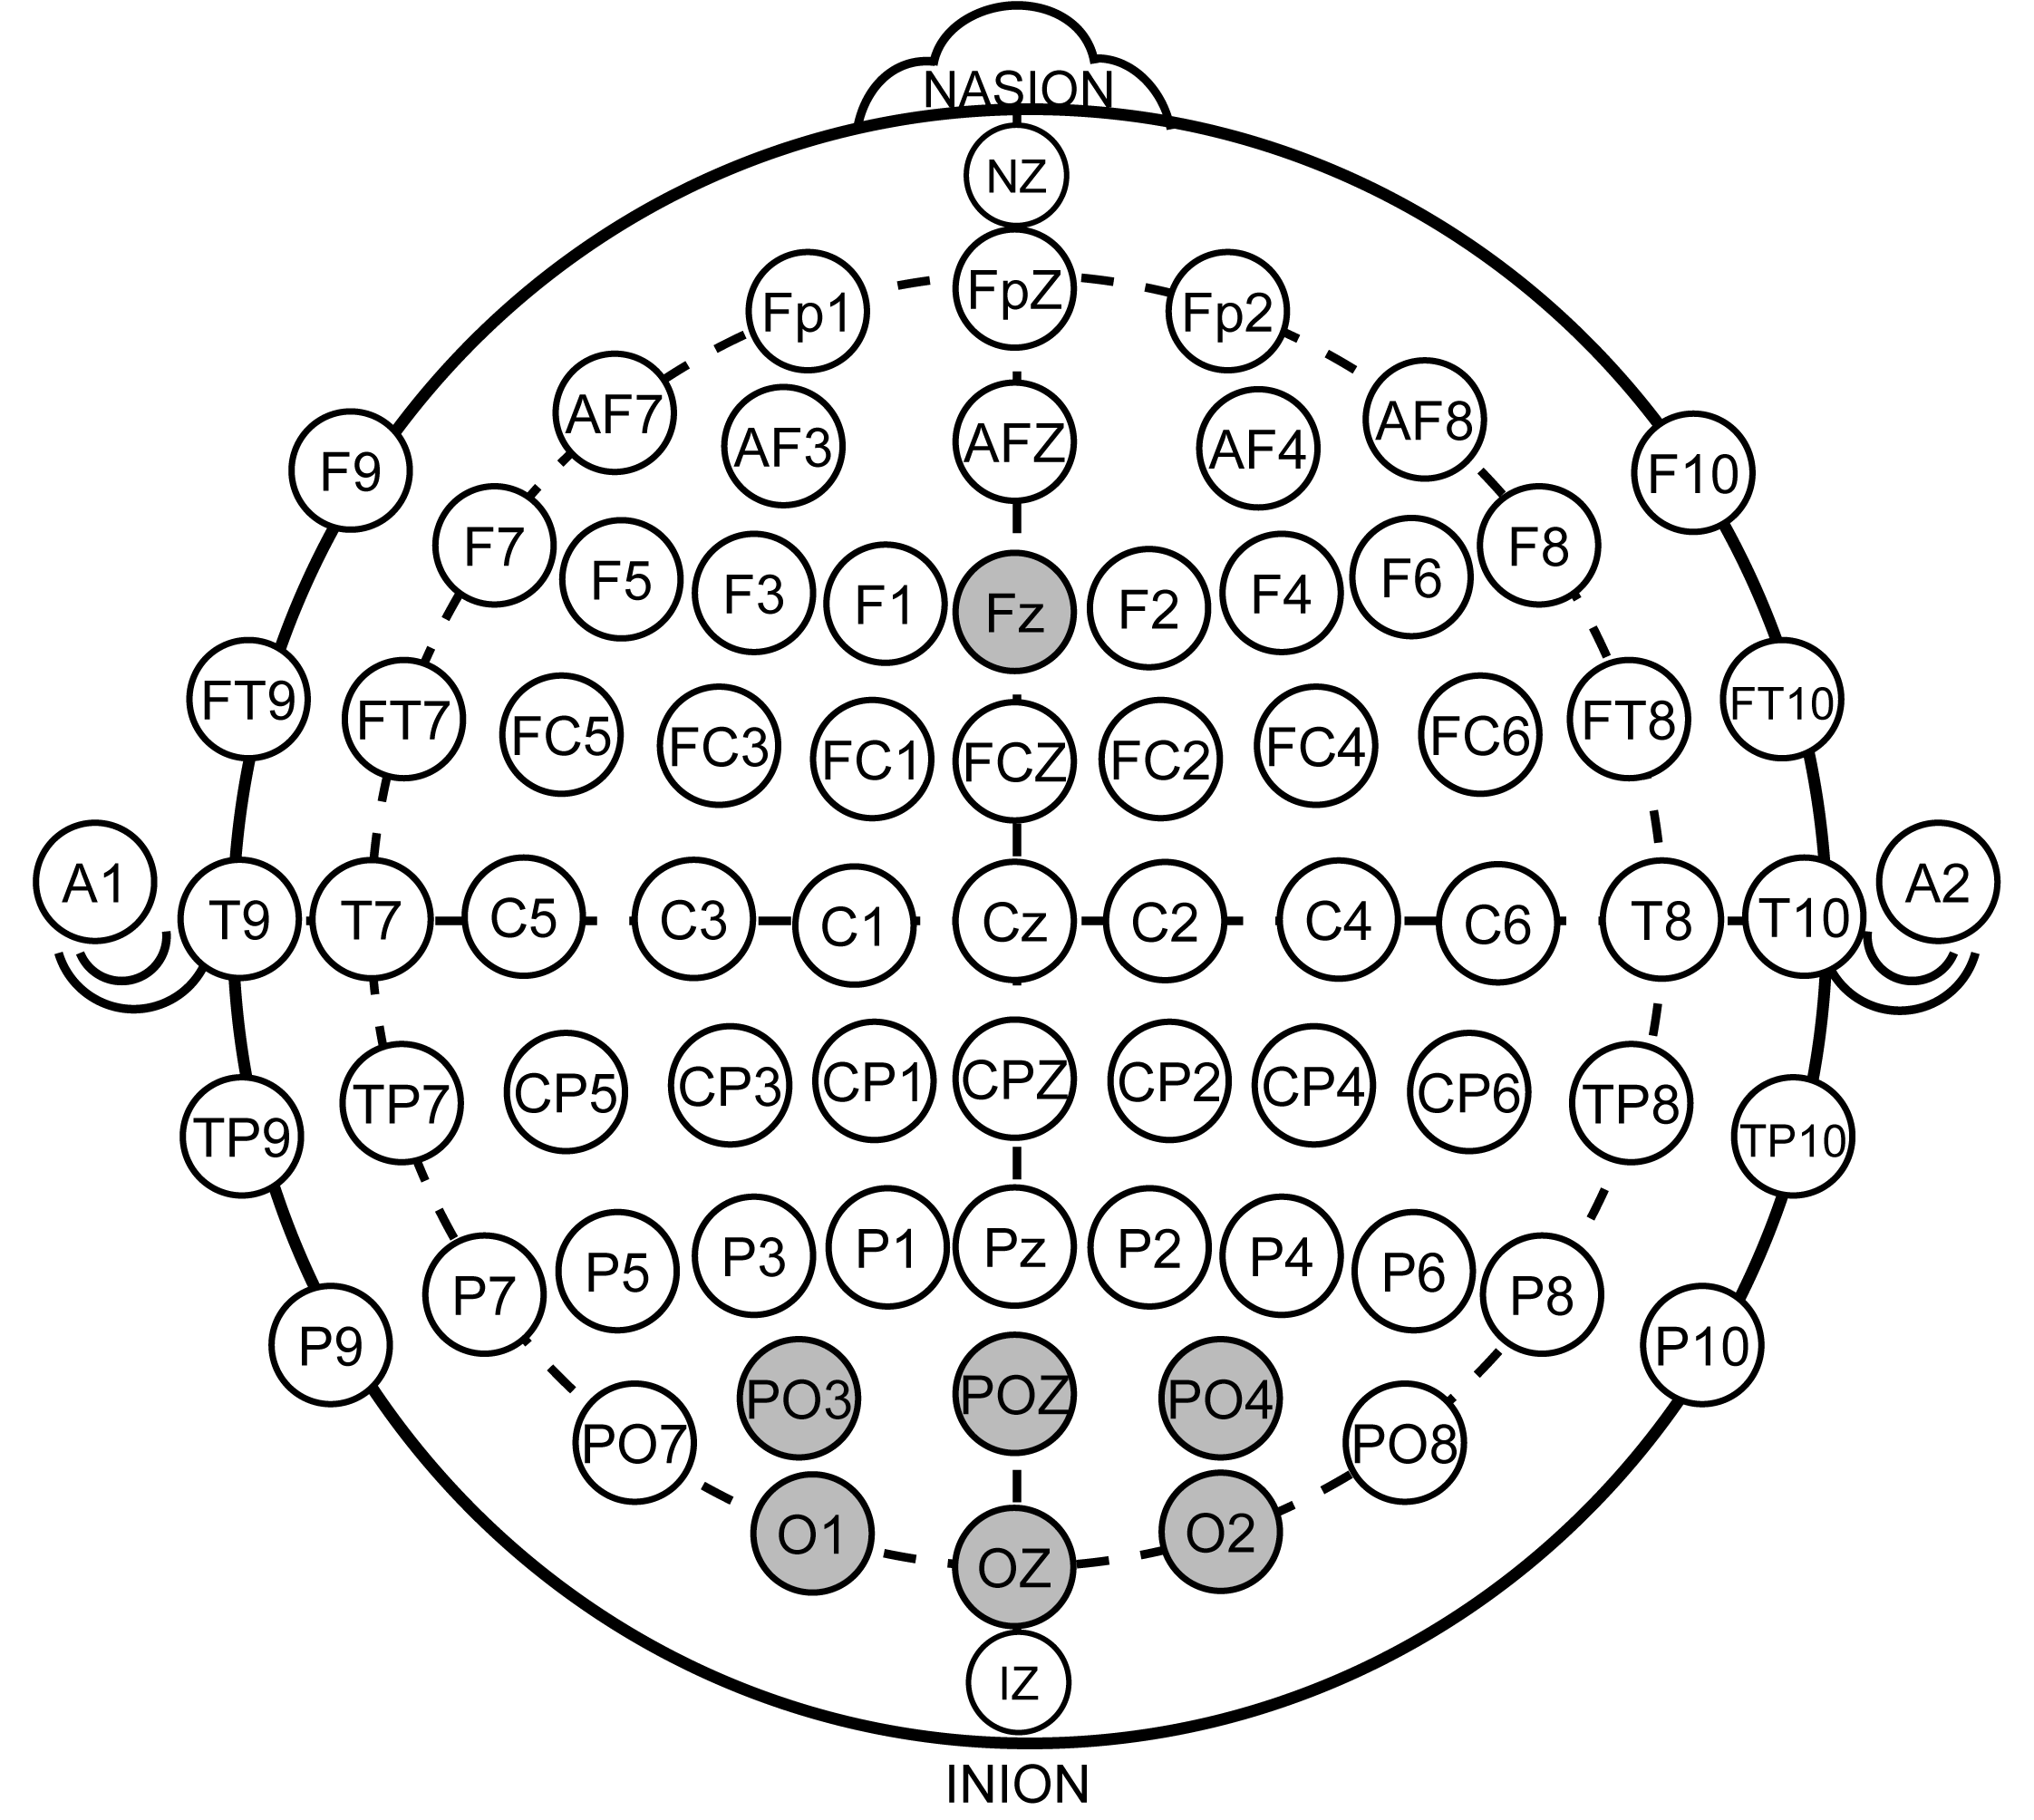
\includegraphics[width=0.45\textwidth]{images/methods/EEG-1020.png}
    \caption{EEG 10--20 System, highlighting the six electrodes and the ground reference used.}\label{fig:EEG-1020}
\end{figure}

Six of the eight electrodes were placed based on the international 10--20 system, specifically on the PO3, POz, PO4, O1, Oz, and O2 channels as illustrated in Figure~\ref{fig:EEG-1020}, while the ground electrode was placed on Fz. The remaining two electrodes were not used due to technical issues. Conductive gel was applied to ensure proper contact between the electrodes and the scalp, which resulted in optimal signal quality. The entire EEG setup process, including electrode placement and application of conductive gel, took approximately 45--60 minutes.

The EEG data was recorded and stored at a sampling rate of 250 Hz using a Python script with the Mentalab library. The refresh rate of the VR screens were set at the maximum of 90 Hz.

% add figure 
\begin{figure}[ht]
    \centering
    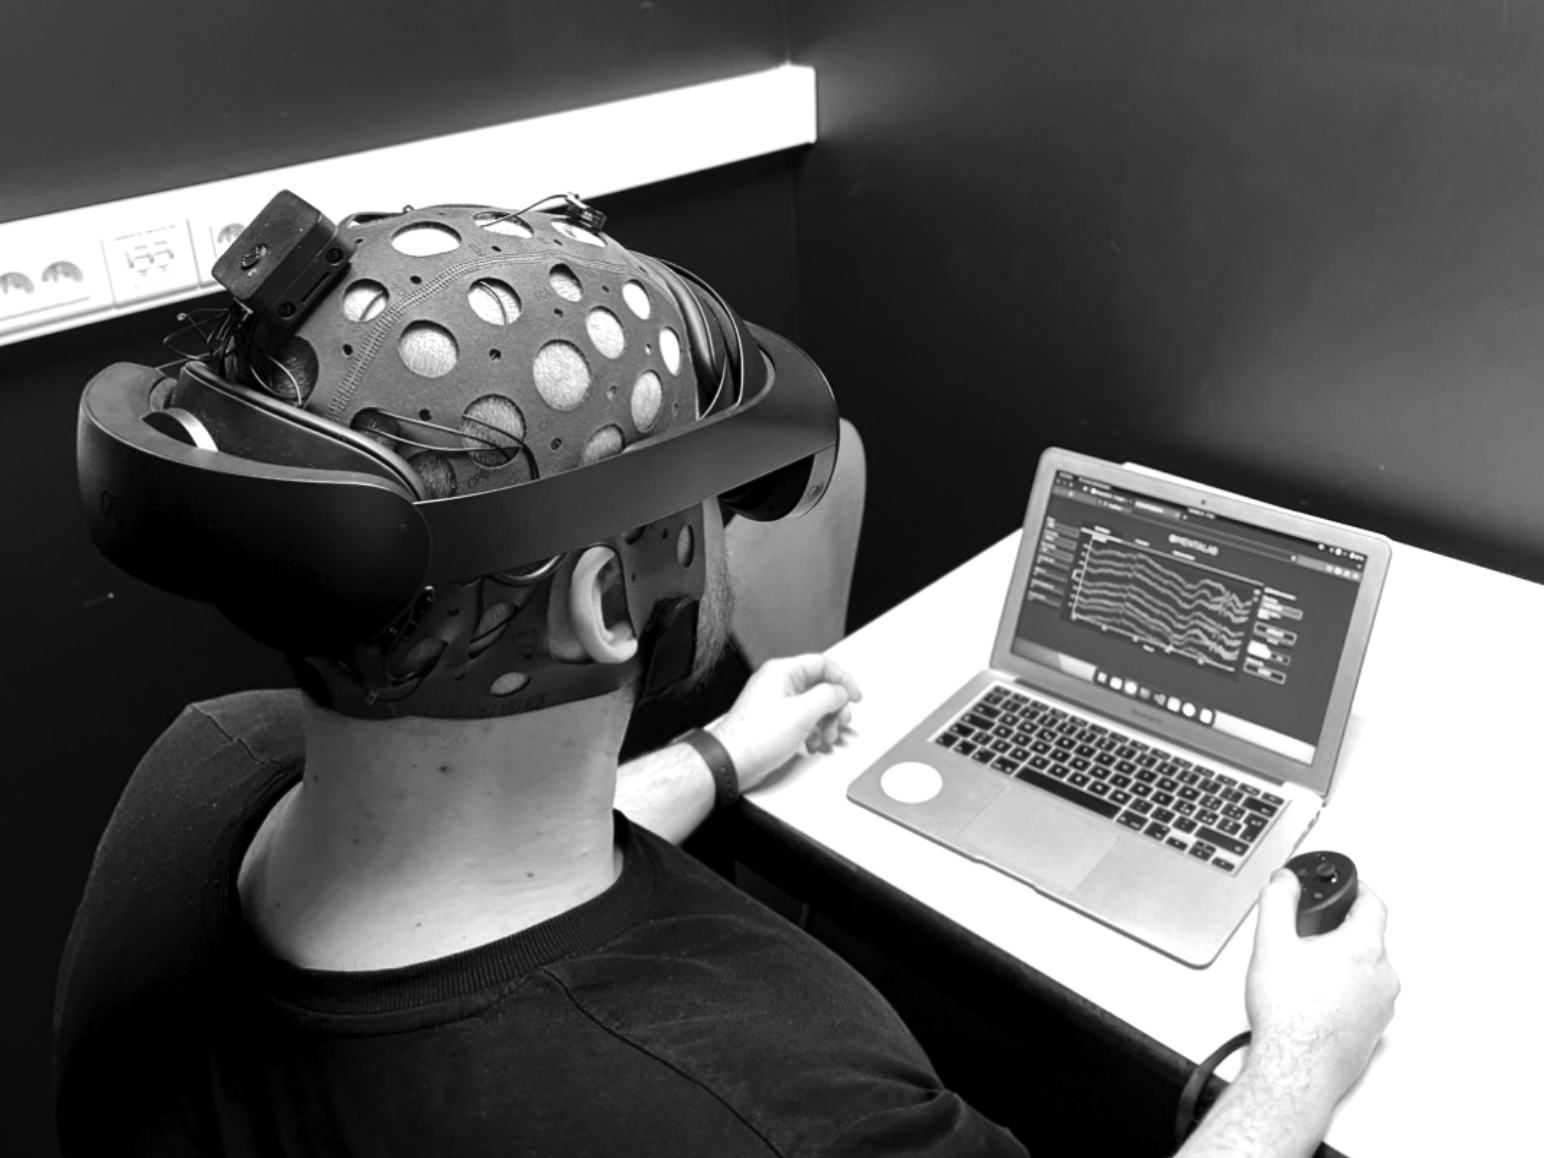
\includegraphics[width=0.5\textwidth]{images/experiments/experiment_setup.png}
    \caption{Experimental setup configuration depicted in the image. The VR controller is on the right hand, on top of the table to minimise movement.}\label{fig:mentalab}
\end{figure}

\section{Application Design}

The application design consists of two main components: the VR Experiment Application and the Transmission Control Protocol (TCP) Server. This allows easy communication and accurate markers synchronization between the VR headset, the laptop server, and the Mentalab system, using the TCP and Lab Streaming Layer (LSL) protocols.

\subsection{VR Experiment Application}


\begin{figure}[b]
    \centering
    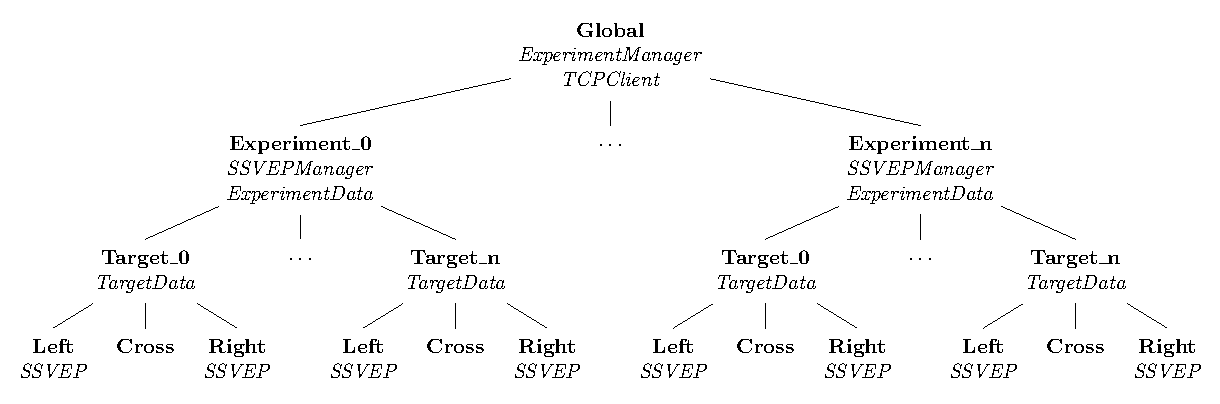
\includegraphics[width=\textwidth]{images/methods/hierarchy.pdf}
    \caption{Unity Scene for the VR Application, with the GameObjects in bold and their Scripts in italics.}\label{fig:unity-scene}
\end{figure}



The VR Experiment Application is a Unity project designed for Meta Quest devices, which comprises multiple experiments with multiple targets. The application is managed by a Global GameObject that communicates with the server through TCP/IP, allowing for the exchange of data, including markers, from the VR application to the laptop server in real-time. The application consists of several components, as illustrated in Figure~\ref{fig:unity-scene}. \\

The game objects are as follows:

\texttt{- Global}: Responsible for the TCPCLient and ExperimentManager scripts.

\texttt{- Experiment}: Responsible for the ExperimentData and SSVEPManager scripts.

\texttt{- Target}: Contains the Left and Right game objects.

\texttt{- Left/Right}: These are the patterns that flicker at the specified frequency. Left is presented to the left eye, and right is presented to the right eye.

\texttt{- Cross}: The cross guides the participant's gaze to the center of the target. 
\\

The scripts are as follows:

\texttt{- TCPClient}: Establishes the TCP connection and manages the communication.

\texttt{- ExperimentManager}: Cycles through the experiments.

\texttt{- ExperimentData}: Manages the experiment's visibility and the target status.

\texttt{- SSVEPManager}: Controls the start and pause of SSVEP components.

\texttt{- TargetData}: Manages the visibility of the Cross object within each target.

\texttt{- SSVEP}: Controls the flickering using a square wave with the specified frequency, as illustrated in Figure~\ref{fig:SSVEP}.

\begin{figure}[ht]
    \centering
    \includegraphics[width=0.65\textwidth]{images/methods/SSVEP.pdf}
    \caption{Black and white checkerboards contrast reversed at 6.6Hz with a square wave (adapted from the supplemental information of~\cite{ZHANG2011362}).}
    \label{fig:SSVEP} 
\end{figure}

\subsection{TCP Server and LSL Integration}

The TCP Server is a Python-based server that listens for client connections on a specific IP address and port. Once the data is received by the laptop server, it is then parsed, and forwarded to the EEG system using the LSL~\cite{lsl} protocol. LSL is an open-source networked middleware ecosystem designed to synchronize various experimental recording streams, including neural data. This protocol is also supported by the Mentalab system.

The markers consisted of a three-digit code. The first digit indicated whether the SSVEP was resumed (1) or paused (2). The second digit represented the experiment number, and the third digit denoted the target within the experiment, starting from the left. For example, 110 corresponded to the start of the leftmost target in the second experiment.

\section{Experiment Design}
In total, four experiments were designed to investigate the research questions in Table \ref{tab:comparisons}. The experiments included multiple targets with different frequencies, presented separately to the left and right eyes. The stimulus pattern design was developed based on previous studies \cite{ZHANG2011362, DavidCarmel2010, yan2011right, hwang2013new, vialatte2010steadystate}, ensuring optimal stimulation of the visual cortex. This included the checkerboard design, the use of a square wave instead of sine, and the color of the checkerboards for the binocular rivalry. 

The stimuli consisted of square wave patterns, with luminance control to maintain consistent brightness. The choice of frequencies (6.6 Hz and 7.5 Hz) was based on previous studies, which have demonstrated their effectiveness in eliciting robust SSVEP responses. Each experiment followed a similar structure of 6-second SSVEP periods and 3-second breaks, repeated ten times per target for a total duration of 90 seconds per target. 


\subsubsection{Experiment 1}
This experiment involved three targets: left, middle, and right, each displaying a black and white checkerboard pattern with the contrast reversed at 7.5 Hz ($f_{1}$) using a square wave, similar to the Figure~\ref{fig:SSVEP}. The left target was visible to the left eye only (L$f_{1}$R$\varnothing$), the middle target was visible to both eyes (L$f_{1}$R$f_{1}$), and the right target was visible to the right eye only (L$\varnothing$R$f_{1}$). 

The objective was to determine if SSVEP responses could be differentiated based on which eye saw the target (left, right, or both) and if it was possible to discern which eye saw it. If successful, this approach could enable the use of three targets with just one frequency.


\begin{figure}[h]
    \centering
    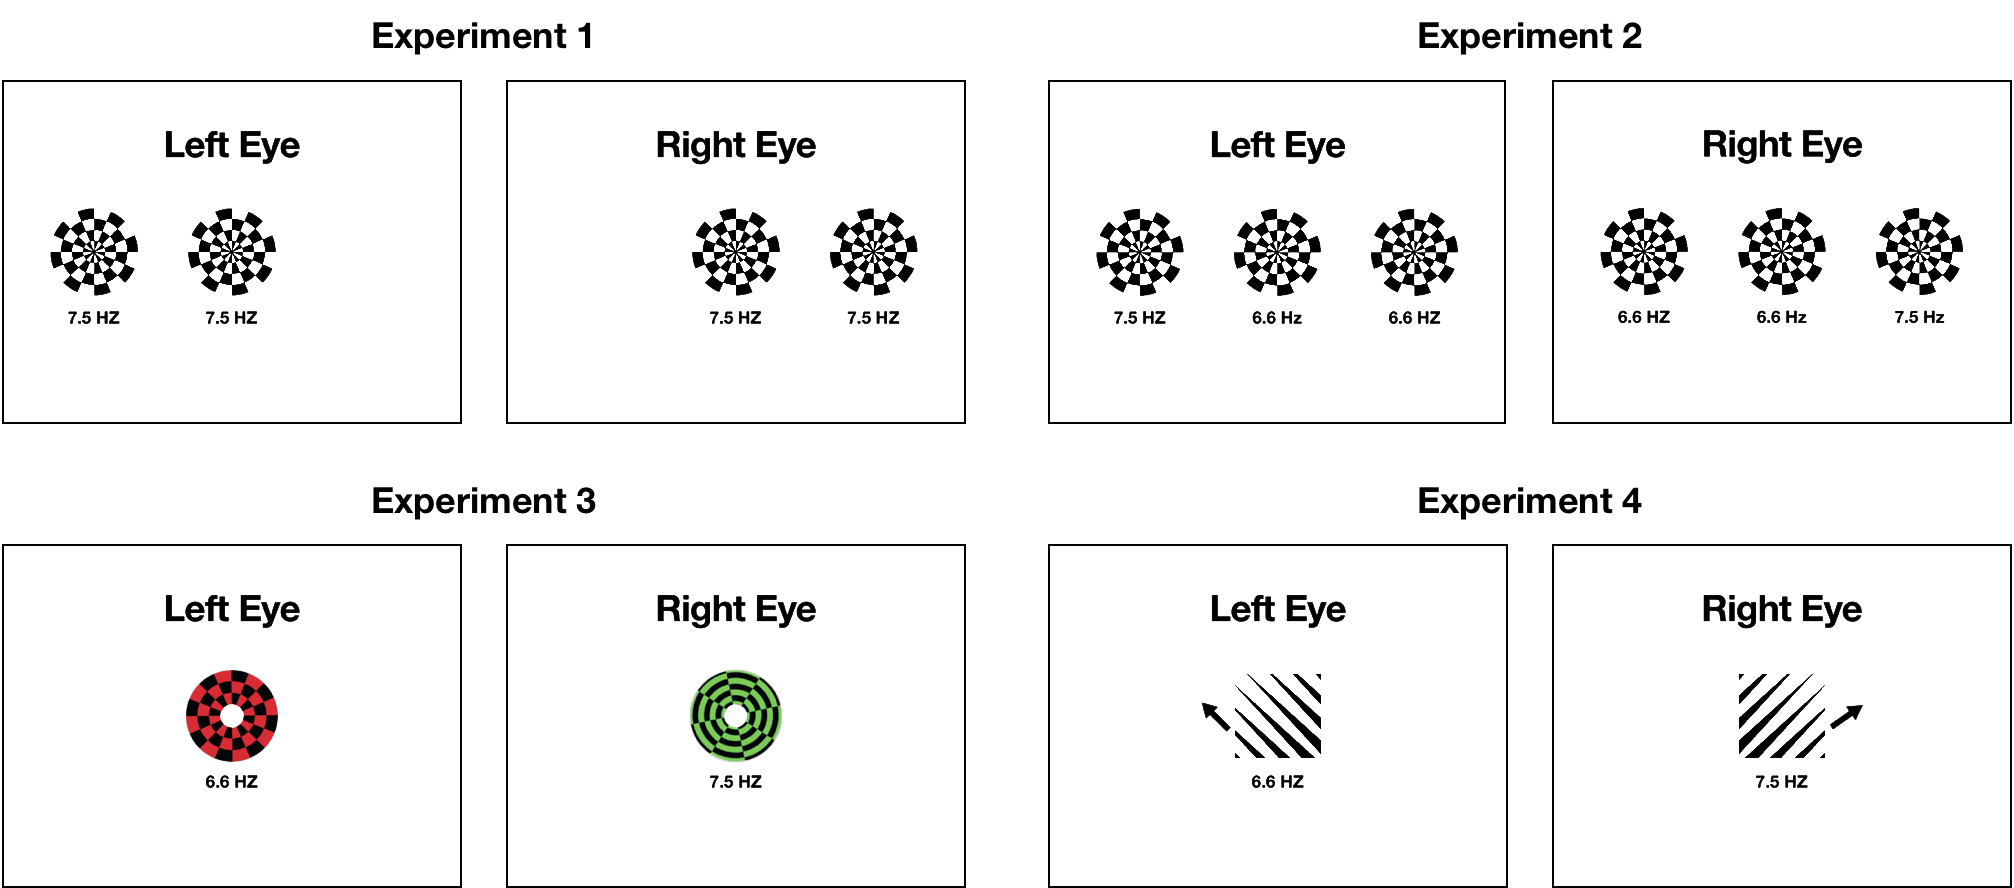
\includegraphics[width=1.0\textwidth]{images/experiments/experiments_w.png}
    \caption{Experiment Guide.}
    \label{fig:experiments}
\end{figure}

% insert figure
\begin{figure}[h]
    \centering
    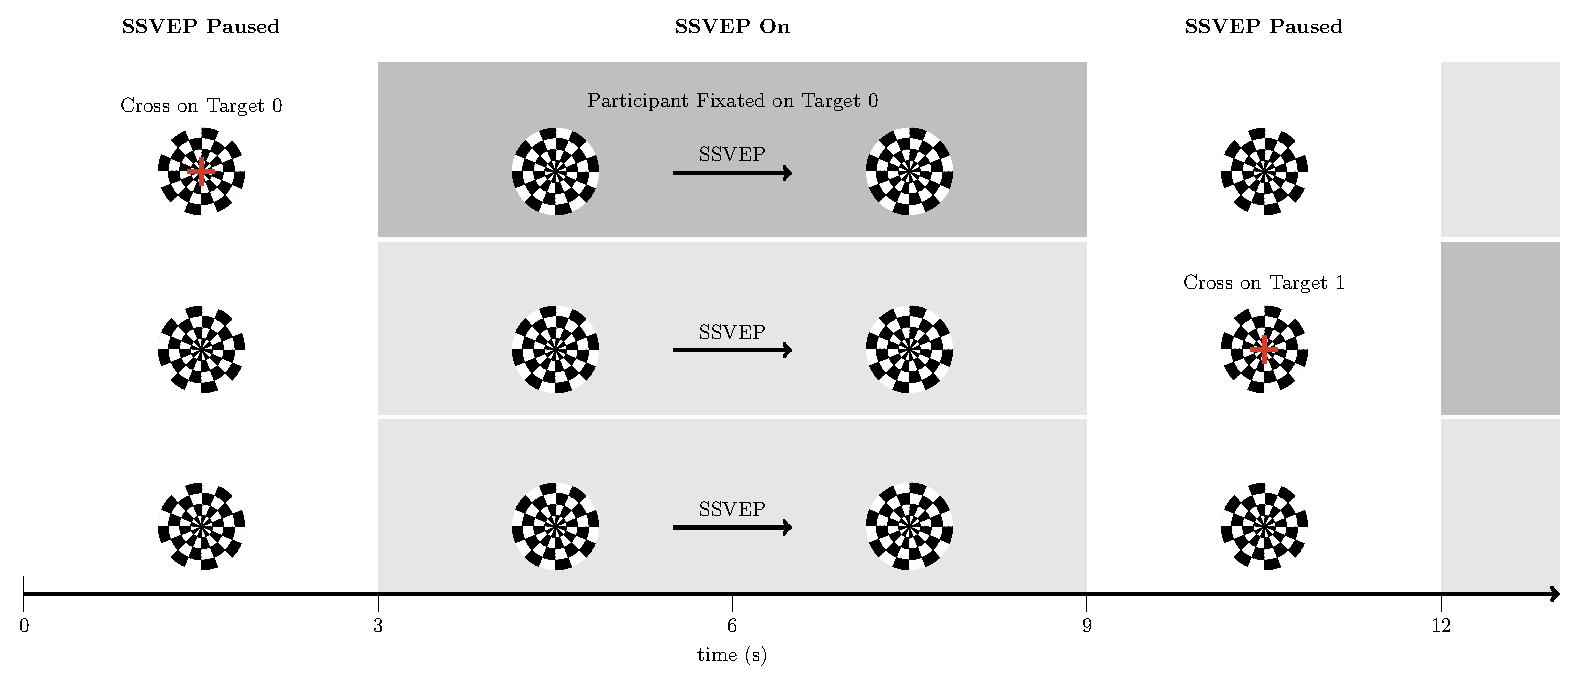
\includegraphics[width=1.0\textwidth]{images/methods/timing.pdf}
    \caption{Illustration of the Timing Graphs for Experiment 1 and Experiment 2.}
    \emph{Throughout this process, we cycled through the patterns illustrated in the figure in a circular manner, conducting 10 trials for each target. A trial was defined as the period between 3 and 9 seconds after the initial appearance of the cross above the respective target. The three targets were positioned side by side, as shown in Figure~\ref{fig:experiments}}
    \label{fig:experiment-timing}
\end{figure}

\subsubsection{Experiment 2}
In this experiment, three targets were presented: left, middle, and right, each displaying a black and white checkerboard pattern. For the left target, the left eye viewed the pattern at 7.5 Hz ($f_{1}$), while the right eye perceived it at 6.6 Hz ($f_{2}$). Conversely, for the right target, the left eye viewed the pattern at $f_{2}$, and the right eye at $f_{1}$. The middle target acted as a reference, flickering at $f_{2}$ for both eyes, in contrast to Experiment 1, where the middle target flickered at $f_{1}$ for both eyes.

The objectives of this experiment were twofold: first, to examine whether the left target (L$f_{1}$R$f_{2}$) could be distinguished from the right target (L$f_{2}$R$f_{1}$) based on the frequency differences perceived by each eye. Second, to assess if two separate SSVEP responses could be simultaneously elicited in both hemispheres. Experiment 2 expands upon Experiment 1, which involved one frequency in one eye and nothing in the other eye.

\subsubsection{Experiment 3}

This experiment served as a preliminary test to assess the feasibility of inducing binocular rivalry in a virtual reality setting. Inspired by the study "Binocular Rivalry Requires Attention," \cite{ZHANG2011362}, it aimed to examine the role of attention in binocular rivalry by presenting a single target with differing stimuli for each eye. The right eye viewed green checkerboards with the contrast reversed at 6.6 Hz (L$\varnothing$R$f_{2}$), while the left eye saw red checkerboards reversed at 7.5 Hz (L$f_{1}$R$\varnothing$). This experiment served as a foundational building step for the subsequent experiment.

\subsubsection{Experiment 4}

Building on the findings of Experiment 3, this final experiment aims to expand on the work done by the paper "Binocular Rivalry Requires Attention" \cite{ZHANG2011362}. Specifically, it assesses the impact of directed attention on binocular rivalry. Participants were instructed to focus on a specific image, as indicated by an arrow pointing in one of the pattern directions during the three-second break before each trial.

In this experiment, a single target was presented, featuring a pattern with white and black spikes rotated at 45 degrees. The spikes were thicker in the middle than on the sides. The left eye viewed the pattern at 6.6 Hz (L$f_{2}$R$\varnothing$), while the right eye saw the same but mirrored pattern at 7.5 Hz (L$\varnothing$R$f_{1}$).

\clearpage
\begin{figure}
    \centering
    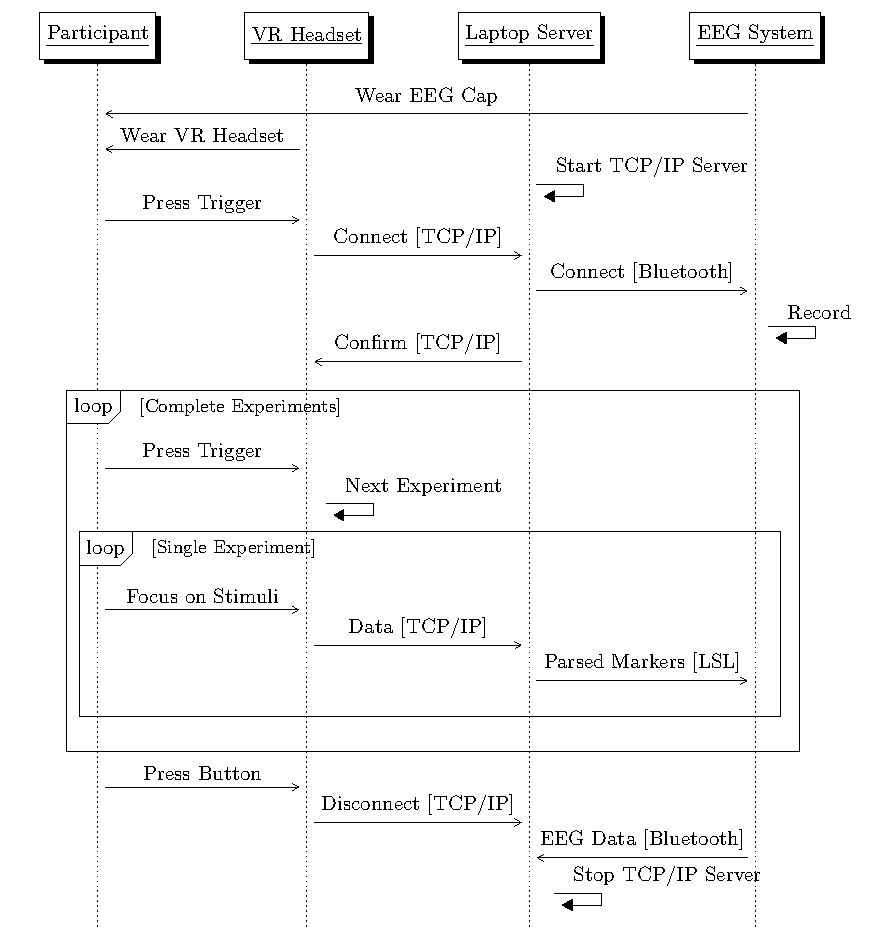
\includegraphics[width=1\textwidth]{images/methods/procedure.pdf}
    \caption{Experimental Procedure.}\label{fig:procedure}
\end{figure}
\clearpage

\section{Experimental Procedure}
Before the experiment, participants were provided with written and verbal instructions explaining the tasks they would perform during the experiment. They were informed about the use of the VR headset and the EEG cap, as well as the purpose of the study. Participants were encouraged to ask questions and clarify any concerns before the experiment began.

The experimental procedure, as illustrated in Figure~\ref{fig:procedure}, consists of several steps involving the participant, the VR headset, the laptop server, and the EEG system. The sequence diagram provides a visual representation of the interaction between these components. Participants were fitted with an EEG headset, followed by wearing the VR headset after ensuring a high-quality clean signal. The TCP server was initiated in the laptop. Participants initiated the connection by pressing the index trigger of the VR controller. A confirmation was sent from the laptop server once both the participant and the researchers were ready.

During the experiment, participants were instructed to focus on flickering stimuli, without moving their head or jaw. Upon completion of each experiment, the participant pressed the trigger to begin the next experiment. This process was repeated until all experiments were completed. The entire procedure was then repeated again. 

Participants were given short breaks of one to three minutes between experiments to minimize fatigue and maintain their focus throughout the experiment. The total duration of the experiment, including breaks, was approximately 45 minutes.

Upon completion of the experiment, participants were given a brief questionnaire to gather subjective feedback on their experience with the VR environment, their ability to focus on the stimuli, and any discomfort or adverse reactions they may have experienced during the experiment.

\section{Data Analysis}

\subsection{Preprocessing}

The signals from the six electrodes were filtered using a fourth-order Butterworth bandpass filter from 3 Hz to 100 Hz. Common average referencing was applied to remove common noise sources by subtracting the average value of all channels from each individual channel. The signals were standardized, centering them around zero mean and scaling them to have a unit standard deviation. Finally, the signals were segmented into epochs based on the event markers.

\subsection{Statistical Analysis}

The statistical analysis aimed to differentiate between SSVEP responses under different experimental conditions. To assess the significance of the observed differences, a significance level of $\alpha=0.05$ was used for all tests. 

The Wilcoxon signed-rank test, a paired test, was utilized to determine whether there existed a significant distinction between two related samples. This test is particularly appropriate when the data deviate from a normal distribution. 

The null hypothesis assumed that the median difference between the two samples was zero. The alternative hypothesis posited that the median difference was not zero.

\subsubsection{Experiment 1 Statistical Analysis}

To assess the differentiation of hemisphere-specific SSVEP responses based on the visually stimulated eye, a comparative analysis of SSVEP response amplitudes at a frequency of 7.5 Hz was conducted. The outcomes were subjected to statistical analysis using the Wilcoxon test, which is appropriate for non-parametric data. The analysis focused on three stimulation conditions: L$f_{1}$R$\varnothing$ vs. L$f_{1}$R$f_{1}$, L$f_{1}$R$\varnothing$ vs. L$\varnothing$R$f_{1}$, and L$f_{1}$R$f_{1}$ vs. L$\varnothing$R$f_{1}$. The resulting p-values were compared to a predefined significance level of 0.05. 

\subsubsection{Experiment 2 Statistical Analysis}

The objective of this experiment was to differentiate SSVEP responses based on the unique frequency stimuli presented to each eye. This was achieved by comparing response amplitudes at frequencies $f_{1}$ (7.5 Hz) and $f_{2}$ (6.6 Hz), as well as the ratio of amplitudes ($f_{2}$/ $f_{1}$). Statistical analysis was performed employing the Wilcoxon test.

\subsubsection{Experiment 3 Statistical Analysis}
Statistical analysis was carried out using the t-test on the ratio of signal strengths at 6.6 Hz and 7.5 Hz for the left, middle, and right hemispheres. To determine the difference beetween these paired observations.

\subsubsection{Experiment 4 Statistical Analysis}

Statistical analyses were conducted by comparing signal ratios and response amplitudes between different conditions using the Wilcoxon test. 

